%-----------------------------------------------------------------------------------------------------
%	INCLUSIÓN DE PAQUETES BÁSICOS
%-----------------------------------------------------------------------------------------------------
\documentclass{article}
%-----------------------------------------------------------------------------------------------------
%	SELECCIÓN DE LA FUENTE
%-----------------------------------------------------------------------------------------------------
% Fuente utilizada.
\usepackage{courier}                    % Fuente Courier.
\usepackage{microtype}                  % Mejora la letra final de cara al lector.
%-----------------------------------------------------------------------------------------------------
%	ALGORITMOS
%-----------------------------------------------------------------------------------------------------
\usepackage{algpseudocode}
\usepackage{algorithmicx}
\usepackage{algorithm}
%-----------------------------------------------------------------------------------------------------
%	IMÁGENES
%-----------------------------------------------------------------------------------------------------
\usepackage{float}
\usepackage{placeins}
%-----------------------------------------------------------------------------------------------------
%	ESTILO DE PÁGINA
%-----------------------------------------------------------------------------------------------------
% Paquetes para el diseño de página:
\usepackage{fancyhdr}               % Utilizado para hacer títulos propios.
\usepackage{lastpage}               % Referencia a la última página. Utilizado para el pie de página.
\usepackage{extramarks}             % Marcas extras. Utilizado en pie de página y cabecera.
\usepackage[parfill]{parskip}       % Crea una nueva línea entre párrafos.
\usepackage{geometry}               % Asigna la "geometría" de las páginas.
% Se elige el estilo fancy y márgenes de 3 centímetros.
\pagestyle{fancy}
\geometry{left=3cm,right=3cm,top=3cm,bottom=3cm,headheight=1cm,headsep=0.5cm} % Márgenes y cabecera.
% Se limpia la cabecera y el pie de página para poder rehacerlos luego.
\fancyhf{}
% Espacios en el documento:
\linespread{1.1}                        % Espacio entre líneas.
\setlength\parindent{0pt}               % Selecciona la indentación para cada inicio de párrafo.
% Cabecera del documento. Se ajusta la línea de la cabecera.
\renewcommand\headrule{
	\begin{minipage}{1\textwidth}
	    \hrule width \hsize
	\end{minipage}
}
% Texto de la cabecera:
\lhead{\subject}                          % Parte izquierda.
\chead{}                                    % Centro.
\rhead{\doctitle \ - \docsubtitle}              % Parte derecha.
% Pie de página del documento. Se ajusta la línea del pie de página.
\renewcommand\footrule{
\begin{minipage}{1\textwidth}
    \hrule width \hsize
\end{minipage}\par
}
\lfoot{}                                                 % Parte izquierda.
\cfoot{}                                                 % Centro.
\rfoot{Page \thepage \ of \protect\pageref{LastPage}} % Parte derecha.


%----------------------------------------------------------------------------------------
%   MATEMÁTICAS
%----------------------------------------------------------------------------------------

% Paquetes para matemáticas:
\usepackage{amsmath, amsthm, amssymb, amsfonts, amscd} % Teoremas, fuentes y símbolos.
\usepackage{tikz-cd} % para diagramas conmutativos
\usepackage{tikz-3dplot}
\tdplotsetmaincoords{0}{0}
\usepackage[mathscr]{euscript}
\let\euscr\mathscr \let\mathscr\relax% just so we can load this and rsfs
\usepackage[scr]{rsfso}
\newcommand{\powerset}{\raisebox{.15\baselineskip}{\Large\ensuremath{\wp}}}
 % Nuevo estilo para definiciones
 \newtheoremstyle{definition-style} % Nombre del estilo
 {5pt}                % Espacio por encima
 {0pt}                % Espacio por debajo
 {}                   % Fuente del cuerpo
 {}                   % Identación: vacío= sin identación, \parindent = identación del parráfo
 {\bf}                % Fuente para la cabecera
 {.}                  % Puntuación tras la cabecera
 {\newline}               % Espacio tras la cabecera: { } = espacio usal entre palabras, \newline = nueva línea
 {}                   % Especificación de la cabecera (si se deja vaía implica 'normal')

 % Nuevo estilo para teoremas
 \newtheoremstyle{theorem-style} % Nombre del estilo
 {5pt}                % Espacio por encima
 {0pt}                % Espacio por debajo
 {\itshape}           % Fuente del cuerpo
 {}                   % Identación: vacío= sin identación, \parindent = identación del parráfo
 {\bf}                % Fuente para la cabecera
 {.}                  % Puntuación tras la cabecera
 {\newline}               % Espacio tras la cabecera: { } = espacio usal entre palabras, \newline = nueva línea
 {}                   % Especificación de la cabecera (si se deja vaía implica 'normal')

 % Nuevo estilo para ejemplos y ejercicios
 \newtheoremstyle{example-style} % Nombre del estilo
 {5pt}                % Espacio por encima
 {0pt}                % Espacio por debajo
 {}                   % Fuente del cuerpo
 {}                   % Identación: vacío= sin identación, \parindent = identación del parráfo
 {\scshape}                % Fuente para la cabecera
 {:}                  % Puntuación tras la cabecera
 {\newline}               % Espacio tras la cabecera: { } = espacio usal entre palabras, \newline = nueva línea
 {}                   % Especificación de la cabecera (si se deja vaía implica 'normal')

 % Teoremas:
 \theoremstyle{theorem-style}  % Otras posibilidades: plain (por defecto), definition, remark
 \newtheorem{theorem}{Theorem}[section]  % [section] indica que el contador se reinicia cada sección
 \newtheorem{corollary}[theorem]{Corollary} % [theorem] indica que comparte el contador con theorem
 \newtheorem{lemma}[theorem]{Lemma}
 \newtheorem{proposition}[theorem]{Proposition}

 % Definiciones, notas, conjeturas
 \theoremstyle{definition-style}
 \newtheorem{definition}{Definition}[section]
 \newtheorem{conjecture}{Conjecture}[section]
 \newtheorem*{note}{Note} % * indica que no tiene contador

 % Ejemplos, ejercicios
 \theoremstyle{example-style}
 \newtheorem{example}{Example}[section]
 \newtheorem{exercise}{Exercise}[section]
 
 \newcommand{\propernormal}{%
  \mathrel{\ooalign{$\lneq$\cr\raise.22ex\hbox{$\lhd$}\cr}}}
  

 % Listas ordenadas con números romanos (i), (ii), etc.
\newenvironment{nlist}
{\begin{enumerate}
\renewcommand\labelenumi{(\emph{\roman{enumi})}}}
{\end{enumerate}}

%commutative-diagrams
\usepackage{tikz-cd}
%-----------------------------------------------------------------------------------------------------
%	BIBLIOGRAFÍA
%-----------------------------------------------------------------------------------------------------

\usepackage[backend=bibtex, style=numeric, sorting = none]{biblatex}
\usepackage{csquotes}

\addbibresource{references.bib}

%-----------------------------------------------------------------------------------------------------
%	PORTADA
%-----------------------------------------------------------------------------------------------------
% Elija uno de los siguientes formatos.
% No olvide incluir los archivos .sty asociados en el directorio del documento.
%\usepackage{title1}
\usepackage{title2}
%\usepackage{title3}

\usepackage{caption}
\usepackage[utf8]{inputenc}

%-----------------------------------------------------------------------------------------------------
%	TÍTULO, AUTOR Y OTROS DATOS DEL DOCUMENTO
%-----------------------------------------------------------------------------------------------------

% Título del documento.
\newcommand{\doctitle}{Equivalences between preadditive categories and certain kinds of rings}
% Subtítulo.
\newcommand{\docsubtitle}{}
% Fecha.
\newcommand{\docdate}{}
% Asignatura.
\newcommand{\subject}{}
% Autor.
\newcommand{\docauthor}{Rodrigo Raya Castellano}
\newcommand{\docaddress}{Universidad de Granada}
\newcommand{\docemail}{}

%-----------------------------------------------------------------------------------------------------
%	RESUMEN
%-----------------------------------------------------------------------------------------------------

% Resumen del documento. Va en la portada.
% Puedes también dejarlo vacío, en cuyo caso no aparece en la portada.
%\newcommand{\docabstract}{}
\newcommand{\docabstract}{}

\begin{document}

\makeatletter\renewcommand{\ALG@name}{Algoritmo}

\maketitle

%-----------------------------------------------------------------------------------------------------
%	ÍNDICE
%-----------------------------------------------------------------------------------------------------

% Profundidad del Índice:
%\setcounter{tocdepth}{1}
\begin{abstract}

\end{abstract}

\newpage
\tableofcontents
\newpage

\section{Preliminaries}
We want to profit of this occasion to give some historical notes that may help future students of the course Modern Algebra in the University of Granada to understand the setting where the two main theories that are studied in the course were developed. 

\subsection{Ring theory}

Many of the initial developments of this theory were motivated by approaches to solve Fermat's Last Theorem. 

\begin{theorem}[Fermat's Last Theorem (1637)]
There do not exist three positive integers $a,b,c$ such
that $a^n+b^n=c^n$ for  an  integer $n$ greater  than  two.
\end{theorem}

Through  attempts  to  prove  this theorem,  the  concept (not the actual name)  of  a  ring  was  introduced  by  Richard  Dedekind  in  the  1800's  as  a  generalization  of  arithmetic. He also coined the terms \textit{ideal} and \textit{module} although the latter was given a much more restricted definition than the modern one \cite{ring}.

It  was  not  until  the  1920's  that  rings
were axiomatically defined by Emmy Noether and Wolfgang Krull in their theory of ideals. Van der Waerden's important work on Modern Algebra contributed to popularize the ideas of Noether who had to face discrimination for being a woman in order to publish her results. 

\begin{figure}[H]
\centering
\begin{minipage}{0.25\textwidth}
\centering
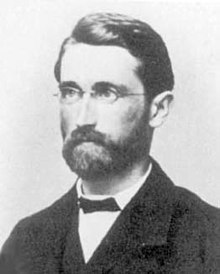
\includegraphics[width=3cm]{images/dedekind.jpeg}
\caption*{Richard Dedekind}
\end{minipage}\hfill
\begin{minipage}{0.25\textwidth}
\centering
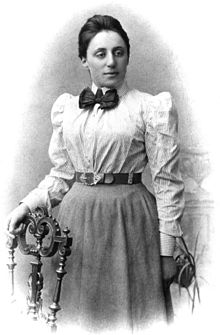
\includegraphics[width=3cm]{images/noether.jpg}
\caption*{Emmy Noether}
\end{minipage}\hfill
\begin{minipage}{0.25\textwidth}
\centering
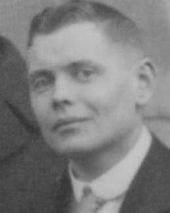
\includegraphics[width=3cm]{images/krull.jpg}
\caption*{Wolfgang Krull}
\end{minipage}\hfill
\end{figure}

Ring theory has since grown to be an active field of research with interesting connections to
algebraic number theory and algebraic geometry.

\subsection{Category theory}

The concept of a category is much younger. It was created  by  Samuel  Eilenberg  and  Saunders  Mac Lane  in
1945 as part of their work in algebraic topology. Applications to other fields of mathematics
have since grown tremendously.  

\begin{figure}[H]
\centering
\begin{minipage}{0.10\textwidth}
\centering
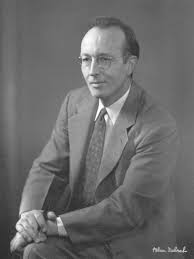
\includegraphics[width=2.5cm]{images/maclane.jpeg}
\caption*{Saunders Mac Lane}
\end{minipage}\hfill
\begin{minipage}{0.10\textwidth}
\centering
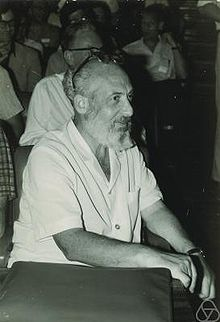
\includegraphics[width=2.5cm]{images/eilenberg.jpeg}
\caption*{Samuel Eilenberg}
\end{minipage}\hfill
\begin{minipage}{0.10\textwidth}
\centering
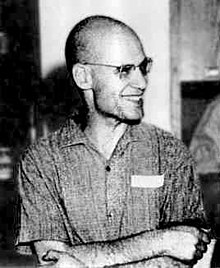
\includegraphics[width=2.5cm]{images/grothendiek.jpeg}
\caption*{Alexander Grothendiek}
\end{minipage}\hfill
\begin{minipage}{0.10\textwidth}
\centering
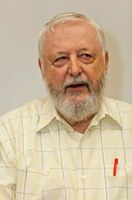
\includegraphics[width=2.5cm]{images/lawvere.jpeg}
\caption*{William Lawvere}
\end{minipage}\hfill
\end{figure}

For instance,  Alexander Grothendieck almost single-handedly shaped modern algebraic geometry. We have read through the biography of Mr. Grothendieck and have been surprised by a life full of difficulties but at the same time full of originality and revolutionary ideas, that we think that is worth commenting here, since it describes best the character of the men that shaped some of the most influential ideas in mathematics. As a motivation for the student to read Récoltes et semailles, we leave the following quote:

\begin{quotation}
Par la suite, j'ai eu l'occasion, dans ce monde des mathématiciens qui m'accueillait, de rencontrer bien des gens, aussi bien des aînés que des jeunes gens plus ou moins de mon âge, qui visiblement étaient beaucoup plus brillants, beaucoup plus "doués" que moi. Je les admirais pour la facilité avec laquelle ils apprenaient, comme en se jouant, des notions nouvelles, et jonglaient avec comme s'ils les connaissaient depuis leur berceau - alors que je me sentais lourd et pataud, me frayant un chemin péniblement, comme une taupe, à travers une montagne informe de choses qu'il était important (m'assurait-on) que j'apprenne, et dont je me sentais incapable de saisir les tenants et les aboutissants. En fait, je n'avais rien de l'étudiant brillant, passant haut la main les concours prestigieux, assimilant en un tournemain des programmes prohibitifs.

La plupart de mes camarades plus brillants sont d'ailleurs devenus des mathématiciens compétents et réputés. Pourtant, avec le recul de trente ou trente-cinq ans, je vois qu'ils n'ont pas laissé sur la mathématique de notre temps une empreinte vraiment profonde. Ils ont fait des choses, des belles choses parfois, dans un contexte déjà tout fait, auquel ils n'auraient pas songé à toucher. Ils sont restés prisonniers sans le savoir de ces cercles invisibles et impérieux, qui délimitent un Univers dans un milieu et à une époque donnée. Pour les franchir, il aurait fallu qu'ils retrouvent en eux cette capacité qui était leur à leur naissance, tout comme elle était mienne : la capacité d'être seul.
\end{quotation}

Another important application of category theory was given by, William
Lawvere, who applied it to logic, developing the field of categorical logic.This theory has important connections with theoretical computer science. In broad terms, categorical logic represents both syntax and semantics by a category, and an interpretation by a functor. The categorical framework provides a rich conceptual background for logical and type-theoretic constructions. 

Applications  to  abstract  algebra  are  especially
interesting  since  one  can  interpret  various  algebraic  structures  as categories and vice-versa in an effort to study them in an uniform fashion.  By
doing so, one can translate propositions proven in categories into results in their respective
algebraic structures.


In the literature, especially in the field of categorification, one often views a ring together
with a collection of idempotents as a category with an object for each idempotent. This is the
point of view we follow in this work. Our goal is to make the connection between rings
(with idempotents) and categories as precise as possible,  and create a dictionary between
the two points of view.  

In particular, we show how we can view:

\begin{itemize}
\item A ring as a small preadditive
category  with  one  object.
\item An  idempotented  ring  as  a  small  preadditive  category  with
finitely many objects.
\end{itemize}  

We then prove an equivalence of categories between:

\begin{itemize}
\item The category of rings and the category of small preadditive categories with one object.
\item The category of idempotented rings and the category of small preadditive categories
with finitely many objects.
\end{itemize}

We conclude with a proof that:

\begin{itemize}
\item An idempotented ring that contains
no zero divisors and whose characteristic is not two has a complete set of primitive orthogonal
idempotents if and only if its corresponding category is idempotent complete.
\end{itemize} 


\newpage
\section{Definitions}
\subsection{Definitions in ring theory}

\begin{definition}[Notions on rings]
\textbf{Complete set of primitive orthogonal elements}

Let $R$ be a ring and a subset $I = \{e_1, e_2,\ldots, e_n\} \subseteq R$. We call $I$ is a complete set of orthogonal idempotents if:

\begin{enumerate}
\item Every pair of distinct $e_i, e_j$ in $I$ is a pair of orthogonal idempotents.
\item $0_R \in I$.
\item $1_R = e_1 + e_2 + \ldots + e_n$.
\end{enumerate}

If every non-zero idempotent in $I$ cannot be written as the sum of two non-zero idempotents, then it is a complete set of primitive orthogonal idempotents.

\textbf{Idempotented ring}

An idempotented ring is a pair $(R, I)$, where $R$ is a ring and $I$ a complete set of orthogonal idempotents.

\begin{example}[Matrix ring]
Given an idempotented ring $(R,I)$, it is easy to show that the matrix ring:

\begin{figure}[H]
\centering
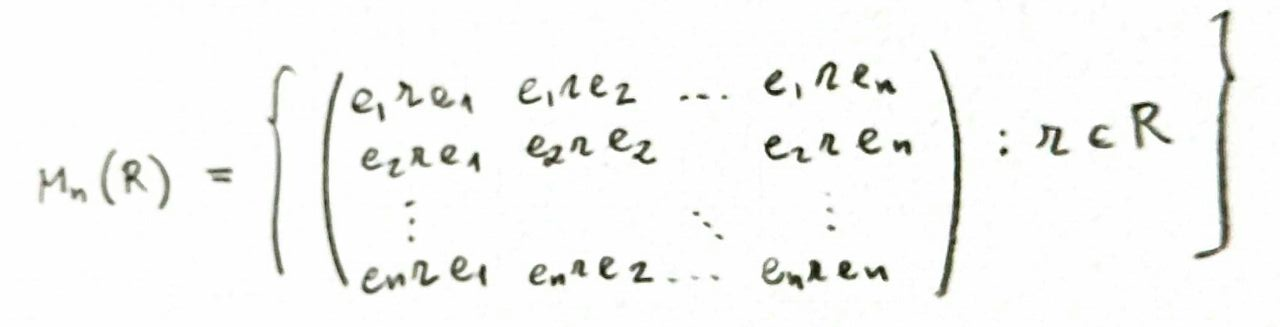
\includegraphics[width=10cm]{images/mring.jpg}
\end{figure}

is also idempotented ring and that every idempotented ring is isomorphic to a matrix ring.
\end{example}

\begin{exercise}[Proposed to the reader]
Prove that $(R,I) \cong (M_n(R),I_{M_n(R)})$. 

Hint: you may use $\phi(r) = (e_jre_i)$ as isomorphism.
\end{exercise}


\textbf{Category of idempotented rings}

The category of idempotented rings, Ring$_\perp$ is given by $Ob(Ring_\perp) = $ idempotented rings and $Mor_{Ring_\perp}((R, I),(S, J)) = $ homomorphisms $h: R \to S$ such that $h(e) \in J$ for all $e \in I$.

Note that this last condition is unnecessary to be mentionned since any ring homomorphism preserves idempotents as: $$e \in I \implies e^2 = e \implies h(e) = h(e)^2 \implies h(e) \in J$$


\end{definition}

\subsection{Definitions in category theory}

\begin{definition}[Notions on categories]

\textbf{Small category}

A category C is small if the class of objects and the class of morphisms are both sets.

\textbf{Preadditive category}

A category $C$ is preadditive if for any $X,Y \in Ob(C)$, $Mor_C(X,Y)$ has the structure of an abelian group, which we write additively. Furthermore, we require that composition is distributive over this addition.

\textbf{Additive functor}

Suppose C and D are preadditive categories. 

A functor $F : C \to D$ is additive if for all $X, Y \in Ob(C), F : Mor_C(X, Y ) \to Mor_D(F (X), F (Y ))$ is a group homomorphism with respect to addition.

\textbf{Category of small preadditive categories with one object}

Let PreCat$_1$ denote the category of small preadditive categories with one object. The objects are small preadditive categories with one object and $Mor_{PreCat_1}(C, D)$ is the class of additive functors from C to D.

\textbf{Category of small preadditive categories with finitely many objects}

Let PreCat$_{Fin}$ denote the category of small preadditive categories with finitely many objects. The objects are small preadditive categories with finitely many objects and MorPreCat$_{Fin}(C, D)$ is the class of additive functors from $C$ to $D$.

\textbf{Split idempotent}

A morphism $e \in Mor_C(X,X)$ is idempotent if $e \circ e = e$.

An idempotent $e$ is an split idempotent if $\exists f \in Mor_C(X,Y), g \in Mor_C(Y,X).g \circ f = e \land f \circ g = id_Y$.


\begin{figure}[H]
\centering
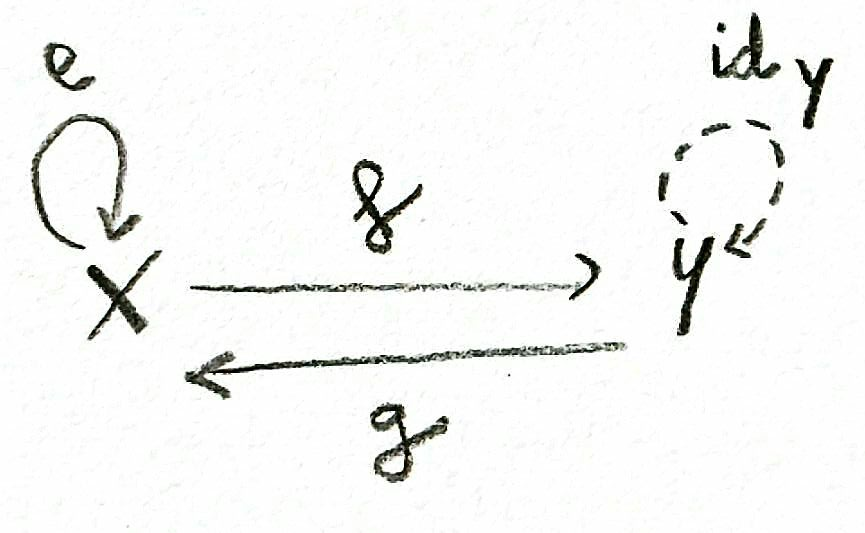
\includegraphics[width=4cm]{images/idempotent.jpg}
\end{figure}

\textbf{Idempotent complete category}

A category $C$ is idempotent complete if every idempotent morphism in $C$ is a split idempotent.
\end{definition}

\begin{definition}[Notions on relations between categories]
Suppose $C$ and $D$ are categories and $F, G: C \to D$ functors. A natural transformation $\eta$ from $F$ to $G$, denoted as $\eta : F \to G$, is a mapping from $Ob(C)$ to $Mor(D)$ that associates every $X \in Ob(C)$ to a morphism $\eta_X \in Mor_D(F(X), G(X))$ such that the following diagram commutes for any $f \in Mor_C(X, Y )$.

\begin{figure}[H]
\centering
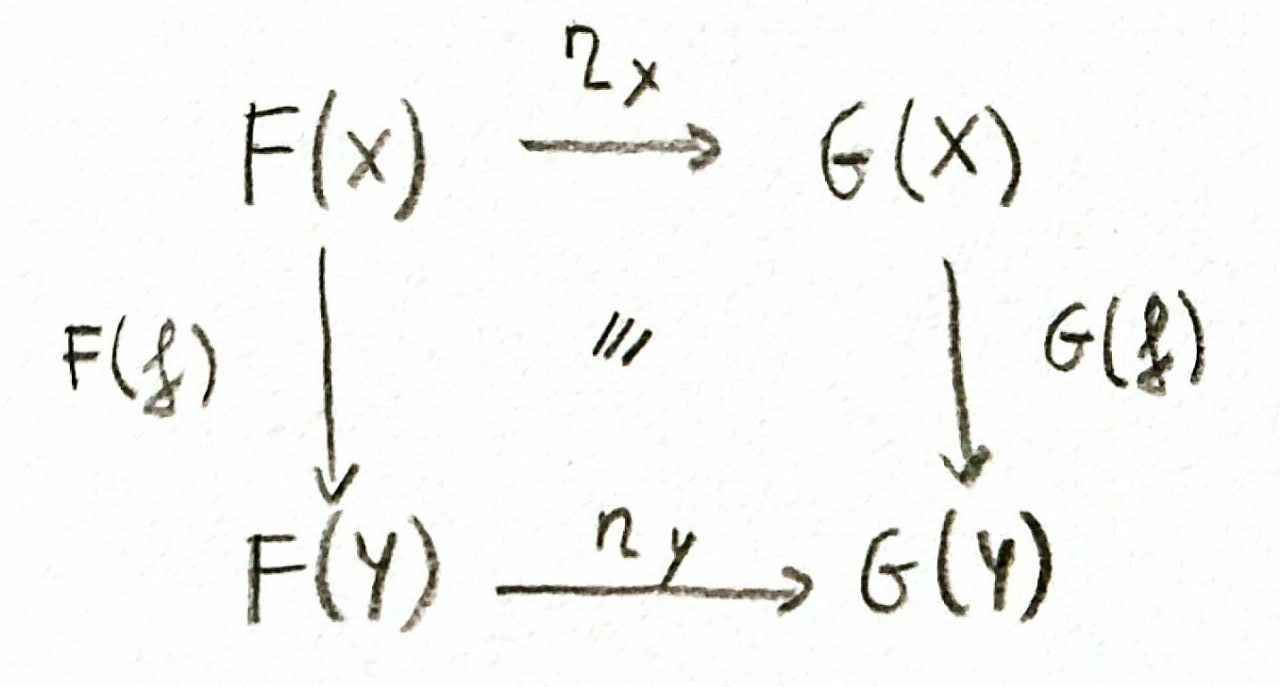
\includegraphics[width=4cm]{images/natural.jpg}
\end{figure}

If $\eta_X:F(X) \to G(X)$ is an isomorphism (there exists an inverse functor) for all $X \in Ob(C)$, then $\eta$ is a natural isomorphism.



\textbf{Equivalence of categories}

Two categories $C$ and $D$ are equivalent (written as $C \simeq D$) if there exists a pair of functors $F : C \to D$, $G: D \to C$ and a pair of natural isomorphisms $\eta: id_C \to G \circ F$, $\epsilon: id_D \to F \circ G$.

Let $C$ and $D$ be categories. Recall that a functor $F : C \to D$ gives rise to map $F_{X,Y} : Mor_C(X,Y) \to Mor_D(F (X), F (Y ))$, for all $X, Y \in Ob(C)$. 

\textbf{Full functor}

The functor $F$ is full on morphisms if $F_{X,Y}$ is surjective for all $X, Y \in Ob(C)$.

\textbf{Faithful functor}

The functor $F$ is faithful on morphisms if $F_{X,Y}$ is injective for all $X, Y \in Ob(C)$. 

\textbf{Fully faithful functor}

If $F$ is both full and faithful, it is called fully faithful.

\textbf{Essentially surjective}

Suppose $C$ and $D$ are categories. A functor $F : C \to D$ is essentially surjective on objects if for all $Y \in Ob(D)$, there exists a $X \in Ob(C)$ such that $F(X) \cong Y $ (objects are isomorphic).

\end{definition}

Equivalences are good because they preserve many (but not every categorical property). Intuitively, one is saying that up to a natural transformation $F,G$ are one the inverse of the other. 

The following result allows to check a list of properties that depend on one morphism instead of proving explicitly the natural transformations.

\begin{theorem}[Maclane]
Suppose $C$ and $D$ are categories and $F : C \to D$ a functor. The functor $F$ yields an equivalence of categories if and only if $F$ is fully faithful on morphisms and essentially surjective on objects.
\end{theorem}





\newpage
\section{Results}
\subsection{The basic equivalences \cite{poon}}

\begin{proposition}[Equivalences between rings and preadditive categories]
We have the following equivalences of categories:

\begin{enumerate}
\item The category Ring is equivalent to the category PreCat$_1$.
\item The category Ring$\perp$ is equivalent to the category PreCat$_{Fin}$.
\end{enumerate}
\end{proposition}
\begin{proof}
Let's see each of the mentioned equivalences:

1. We define a functor $G:PreCat_1 \to Ring$ as: $$G(C) = R_C = Mor_C(*,*)$$ here $*$ is the unique object of the category and given $H \in  Mor_{PreCat_1}(C,D)$ and $r \in Mor_{C}(*,*)$: $$G(H)(r) = H(r)$$ We observe that this is well-defined since $H$ is an additive functor and gives a ring homomorphism.

\textbf{$G$ is a functor}

\begin{itemize}
\item It preserves the identity morphism, $G(id_C)(r) = id_C(r) = r$, so that $G(id_C)$ is the identity ring morphism in $R_C$.
\item It preserves composition, if $C,D,E \in Ob(PreCat_1)$ and we have $H:C \to D,H':D \to E$,$r \in R_C$, then $G(H \circ H')(r) = (H \circ H')(r) = (G(H) \circ G(H'))(r)$.
\end{itemize}  

\textbf{$G$ is fully faithful and essentially surjective}

To ease notation, one introduces the inverse functor of $G$, $F:Ring \to PreCat_1$, such that: $$F(R) = C_R$$ where $C_R$ is the preadditive category given by $Ob(C_R) = \{\star\}$ and $Mor C_R = R$ and for a morphism $h \in Mor_{Ring}(R,S)$, $F(h):C_R \to C_S$ is an additive functor given by: $$F(h)(*) = *$$ $$F(h)(r) = h(r)$$ We leave as an exercise to check that $F(h)$ is indeed a functor. 

\begin{itemize}
\item $G$ is full. For any $h \in Mor_{Ring}(R,S)$ we have that $G(F(h)) = G \circ F(h) = h$. 
\item $G$ is faithful. Assume $G(H) = G(J)$. Necessarily, $G,H$ must me equal on $Ob(C) = \{\star\}$. On morphisms: $$G(H) = G(J) \implies \forall r \in R. G(H)(r) = G(J)(r) \implies \forall r \in R. H(r) = J(r)$$ Therefore, we have that $G = H$.
\item $G$ is essentially surjective.  Let $R \in Ob(Ring)$, then $G(F(R)) = R$.
\end{itemize}  

2. We define a functor $G:PreCat_{Fin} \to Ring_{\perp}$ such that: $$G(C) = (R_C,I_C)$$ where $R_C = \oplus_{X,Y \in Ob(C)} Mor_C(X,Y)$ is a ring and $$I_C = \{id_X:X \in Ob(C)\}$$ is a complete set of orthogonal idempotents. The representation of this ring ca be done as in the following figure:  \begin{figure}[H]
\centering
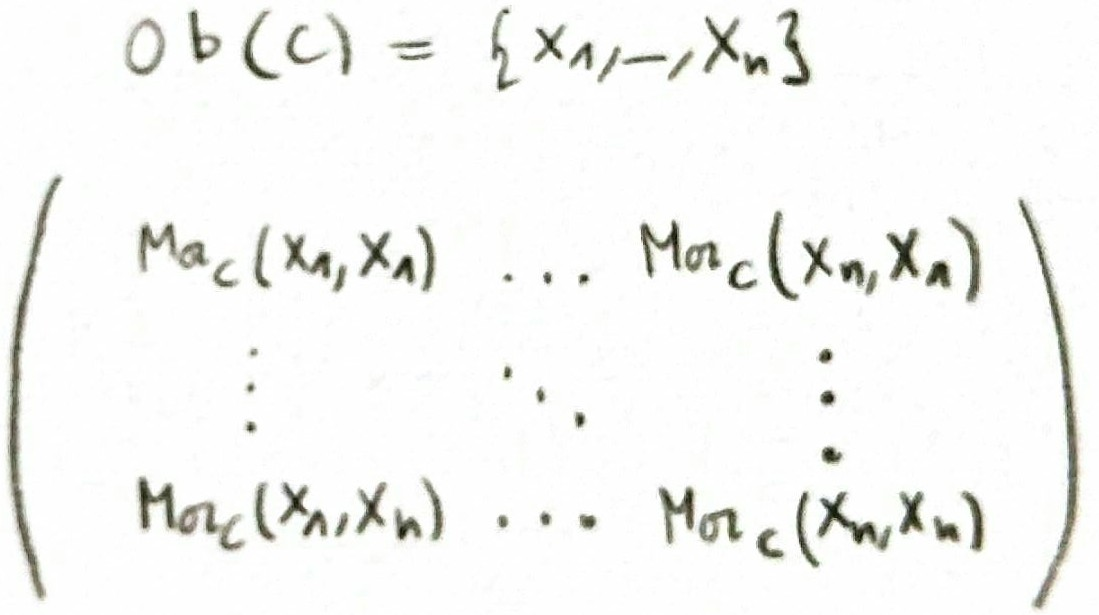
\includegraphics[width=4.5cm]{images/matrix.jpg}
\end{figure} where the order in the indexes is determined for matrix multiplication to compose well the morphisms. The representation of the orthogonal idempotents would be then: \begin{figure}[H]
\centering
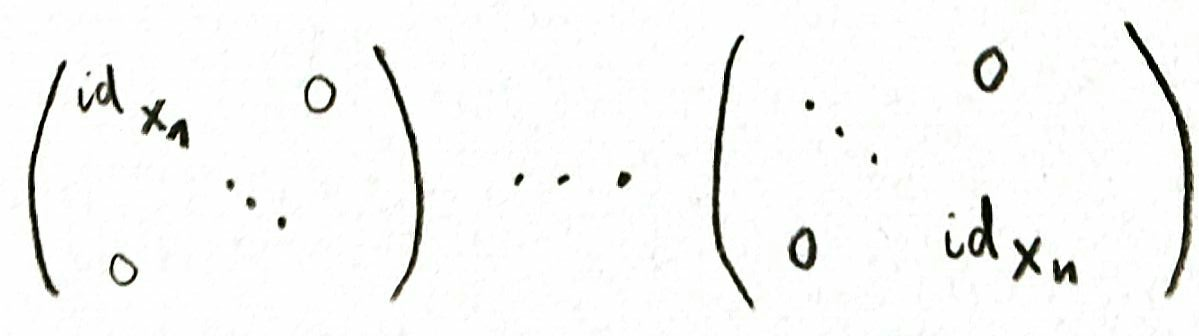
\includegraphics[width=6cm]{images/idem.jpg}
\end{figure}

We leave as an exercise to check that indeed $(R_C,I_C)$ is an idempotented ring. 

Then, for an additive functor $H$ we define: $$G(H)\Big(\sum_{X,Y \in Ob(C)} f_{X,Y}\Big) = \sum_{X,Y \in Ob(C)} H(f_{X,Y})$$ 

\textbf{$G$ is a functor}

\begin{itemize}
\item It preserves the identity morphism since: 

$G(id_C)(\sum_{X,Y} f_{X,Y}) = \sum_{X,Y \in Ob(C)} id_C(f_{X,Y}) = \sum_{X,Y \in Ob(C)} f_{X,Y} = id_{G(C)}(\sum_{X,Y \in Ob(C)} f_{X,Y})$
\item It preserves composition of morphisms since given $C,D,E \in Ob(PreCat_{Fin})$ with morphisms $H:C \to D,H':D \to E$, we have that:

$G(H \circ H')(\sum_{X,Y \in Ob(C)} f_{X,Y}) = \sum_{X,Y \in Ob(C)} H' \circ H(f_{X,Y}) = G(H') \circ  G(H)(\sum_{X,Y \in Ob(C)} f_{X,Y})$.
\end{itemize}

\textbf{$G$ is fully faithful and essentially surjective} 

\begin{itemize}
\item $G$ is full. If $h \in Mor_{Ring_\perp}((R_C,I_C),(R_D,I_D))$ and we take $H \in Mor_{PreCat_{Fin}}(C,D)$ such that: $$H(X) = Dom(h(id_X))$$ $$H(f_{X,Y}) = h(f_{X,Y})$$ In this way, $H(F_{X,Y})$ is a morphism from $H(X)$ to $H(Y)$. So we have: $$G(H)\Big(\sum_{X,Y \in Ob(C)} f_{X,Y}\Big) = \sum_{X,Y \in Ob(C)} H(f_{X,Y}) = \sum_{X,Y \in Ob(C)} h(f_{X,Y}) = h\Big(\sum_{X,Y \in Ob(C)} f_{X,Y}\Big)$$ and therefore, $G(H) = h$. 

\item $G$ is faithful. If $H,J \in Mor_{PreCat_{Fin}}(C,D)$ and we assume that $G(H) = G(J)$ then, they are the same ring homomorphism and so in particular they are equal on the idempotents $id_X$ but this implies that they are equal on objects since $ id_{H(X)} = H(id_X)  = J(id_X) = id_{J(X)}$ so $H(X) = J(X)$. 

On morphisms, if $f_{X,Y} \in Mor_C(X,Y)$ then if $(f_{X,Y})$ denotes the matrix with zero entries except for position $(X,Y)$ containing $f_{X,Y}$, then $G(H)(f_{X,Y}) = G(J)(f_{X,Y}) \implies H(f_{X,Y}) = J(f_{X,Y})$. As a consequence, $H = J$. 

\item $G$ is essentially surjective.

For this part, one uses the inverse functor $F:Ring \to PreCat_{Fin}$ such that for $(R,I) \in Ring_{\perp}$ gives: $$F(R) = C_{(R,I)}$$ where $C_{(R,I)}$ is the category with $Ob(C_{(R,I)}) = I$ and $Mor_{C(R,I)}(e_i, e_j) = e_jRe_i$ and for $h \in Mor_{Ring_{\perp}}((R,I),(S,J))$ we have $F(h)$ defined as: $$F(h)(e_i) = h(e_i)$$ for $e_i \in Ob(C_{(R,I)})$ and for $e_ire_j \in Mor_{C_(R,I)}(e_i,e_j)$: $$F(h)(e_jre_i) = h(e_jre_i)$$ we leave as an exercise to show that $F$ is a functor. 

The strategy then to prove essential surjectivity is, given $(R,I) \in Ob(Ring_{\perp})$ where $I = \{e_1,\ldots,e_n\}$ we claim that $G(F(R)) = G \circ F(R) \cong (M_n(R),I_{M_n(R)}) \cong (R,I)$. The second isomorphism is evident an has been presented above. The first isomorphism uses $\phi:(M_n(R),I_{M_n(R)}) \to G(F(R))$ given by $\phi((e_jre_i)) = (\sum_{i,j} e_jre_i)$.
\end{itemize}

\end{proof}

\begin{exercise}[Proposed to the reader]
If we remove the condition of finite number of objects and we generalize the above construction then we would get infinite matrices:

\begin{figure}[H]
\centering
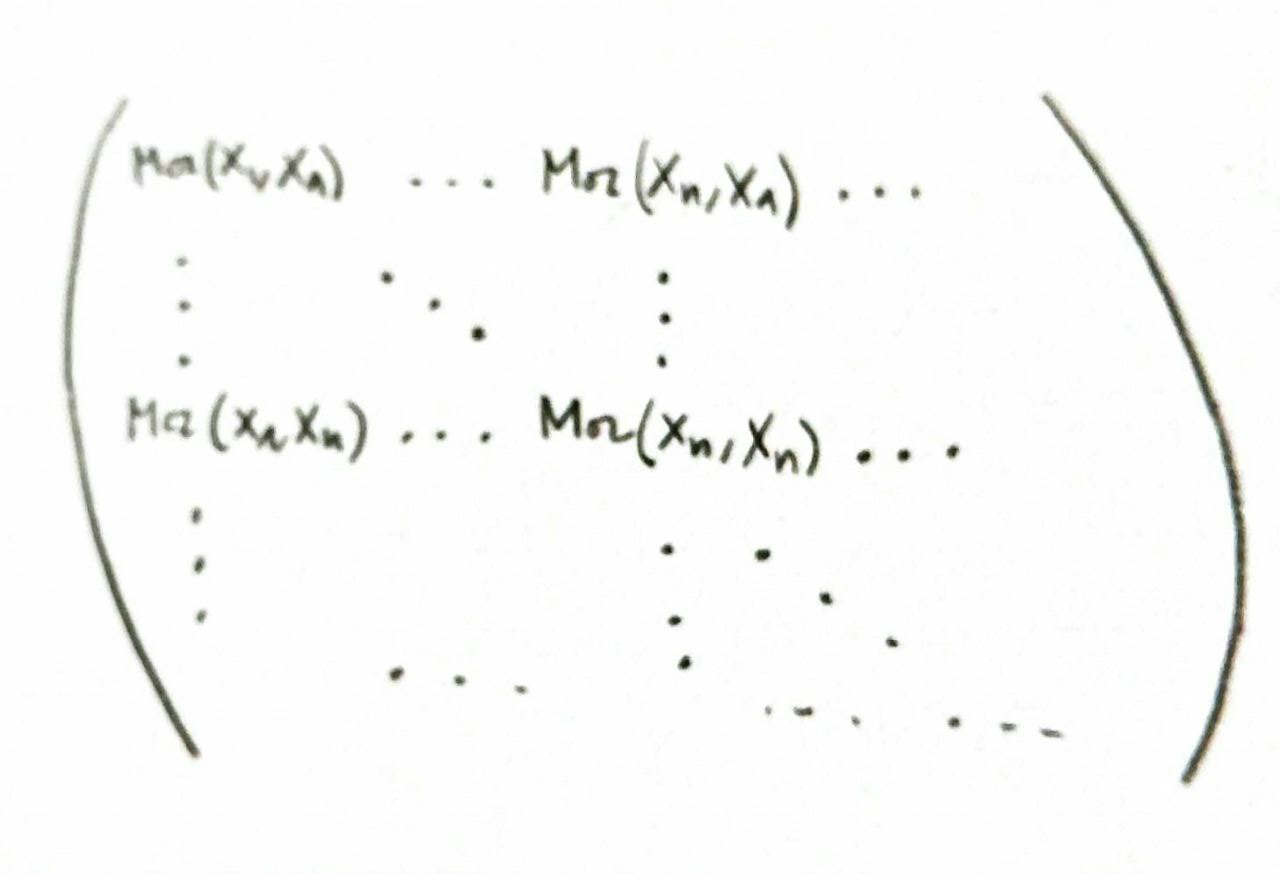
\includegraphics[width=5cm]{images/infinite.jpg}
\end{figure}


that would not have a one (since direct sum has a finite number of non-zero entries):

\begin{figure}[H]
\centering
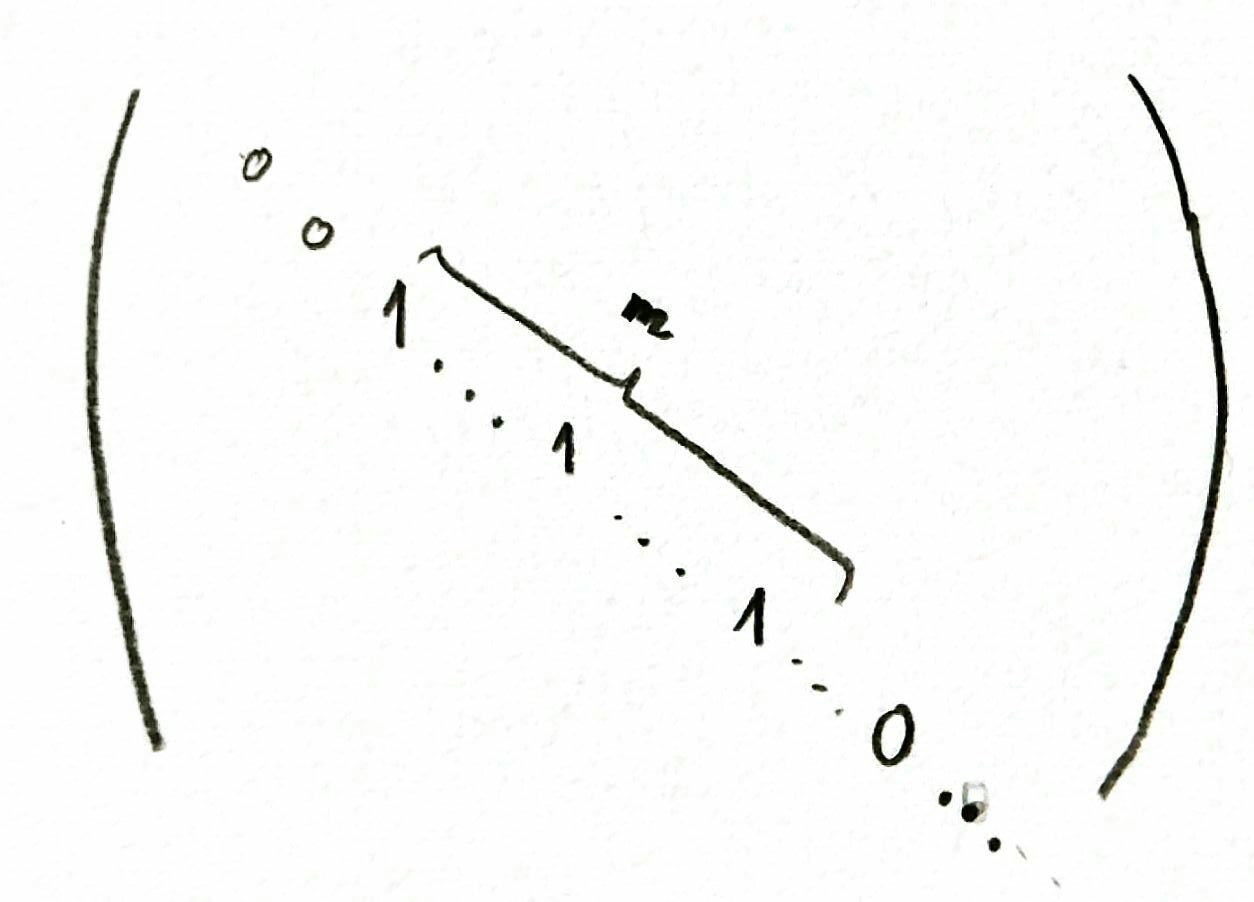
\includegraphics[width=4cm]{images/one.jpg}
\end{figure}

As an exercise, we propose to reader to check if there is an equivalence with rings without one and preadditive categories with an infinite number of objects. 
\end{exercise}

\begin{exercise}[Proposed to the reader]
Can you think of any categorical notion preserved under the equivalences preserved above?

Does this notion provide us with useful theorems about rings, categories or their correspondences?
\end{exercise}

\subsection{Derived results}


\begin{proposition}
Let $(R,I)$ be an idempotented ring that contains no zero divisors and where $Char(R) \neq 2$. Then:

$C_{(R,I)}$ is idempotent complete if and only if $I$ is a complete set of primitive orthogonal idempotents.
\end{proposition}
\begin{proof}
$\implies$ We consider the category $C_{(R,I)}$ as above. We assume that it is idempotent complete. Since we know that $(R,I)$ is an idempotented ring we just have to prove that any non-zero idempotent in $I$ cannot be written as the sum of two non-zero idempotents (not necessarily in $I$). 

Suppose that $e_i = e'+e'' \in I$ where $e',e'' \in I$.  We have to prove that either $e' = 0$ or $e'' = 0$. 

\textbf{$e'$ and $e''$ are pairwise orthogonal}

$e_i = e_i^2 \implies e'+e'' = (e'+e'')^2 = (e'+e'')(e'+e'') = e'e'+e'e''+e''e'+e''e'' = e'+e'e''+e''e'+e''$

$\implies 0_R = e'e''+e''e' \implies e'e''=-e''e' \implies e'e'' = e'e'e''=-e'e''e' \implies e'e''+e'e''e' = 0_R \implies$

 $e'e''(1+e') = 0_R$

Now, since $Char(R) \neq 2$, $(-1)$ is not an idempotent, which implies that $e'e'' = 0_R$. As we wanted. 

\textbf{e'' = 0}

$e'e_ie' = e'(e'+e'')e' = e'e'e'+e'e''e' = e'$ since $e'e'' = 0$. Then, $e_ie'e_i$ is an idempotent as $e_ie'e_i = (e'+e'')e'(e'+e'') = e'$. 

Using that $C_{(R,I)}$ is idempotent complete, we show that, $e_ie'e_i$ is a split idempotent. Indeed, $\exists e_jre_i \in Mor_{C(R,I)}(e_i,e_j),e_ise_j \in Mor_{C(R,I)}(e_j,e_i).e_j = (e_re_i)(e_ise_j) = e_jre_ise_j,e' = e_ie'e_i = (e_ise_j)(e_jre_i) = e_ise_jre_i$. Then we have that:

$e' = e_ise_jre_i =(e'+e'')se_jr(e'+e'') \implies e' = e'e'e' = e'(e'+e'')se_jr(e'+e'')e' = e'se_jre' \implies e'e_ie' = e'se_jre' \implies e'e_ie' - e'se_jre' = 0_R \implies e'(e_i-se_jr)e' = 0_R$

Since $R$ has no zero divisors and $e'$ is nonzero, necessarily, $e_i-se_jr = 0_R \implies e_i = se_jr$. This gives us, $e' = e_ise_jre_i = e_ie_ie_i = e_i$.

Finally, $e_i = e'+e'' \implies e' = e'+e'' \implies e'' = 0_R$. Of course, we have arrived to a contradiction so the implication is complete.

$\Rightarrow$ Assuming $I$ is a complete set of primitive orthogonal idempotents. We take an idempotent morphism $ere \in Mor_{C(R,I)}(e,e)$. We write $e = ere + (e-ere)$ and note that $e-ere$ is an idempotent:

$ \implies (e-ere)(e-ere) = ee - e(ere) - (ere)e + (ere)(ere) = (e-ere)$ 

We have expressed the idempotent $e$ as a sum of two idempotents and since $e$ is in $I$, it is primitive and therefore, $ere = 0$ or $e-ere = 0$. 

If $ere = 0$ then it splits via maps from $0_R$ to $0_R$ ($0$ is an idempotent of the ring). 

If $e-ere = 0$ then $e = ere$ and since $e$ is the identity on $Mor_{C(R,I)}(e,e)$ we can split it as the composition $e \circ e$. 

Therefore, our idempotent $ere$ is a split idempotent and our category is idempotent complete. 
\end{proof}

\begin{exercise}[Proposed to the reader]
Give an interpretation of the above proposition. 

Hint: primitive elements normally imply that decompositions of the ring of the form $R = Re_1 \oplus \ldots \oplus Re_t$ are idecomposable. For instance see the following result taken from \cite{sydney}:

\begin{proposition}
Let $A$ be an $F$-algebra and $e \in A$ an idempotent element. Then $e$ is primitive if
and only if the left ideal $Ae$ is indecomposable.
\end{proposition}

Beware the notions of primitive element may be slightly different!
\end{exercise}

\begin{exercise}[Proposed to the reader]
Does the converse of this proposition hold? That is: 

\begin{proposition}
If $I$ is a complete set of primitive orthogonal idempotents then $(R,I)$ be an idempotented ring that contains no zero divisors and where $Char(R) \neq 2$.
\end{proposition}
\end{exercise}









\newpage


\printbibliography

\end{document}








